\documentclass{beamer}
\mode<presentation> {
    \usetheme{Madrid}
}
\setbeamertemplate{footline}[page number]
\usepackage{graphicx} 
\usepackage{booktabs}
\usepackage{amsmath}
\usepackage{mathtools}
\usepackage[plain]{algorithm}
\usepackage[noend]{algpseudocode}
\usepackage{multicol}

\DeclarePairedDelimiter\ceil{\lceil}{\rceil}
\DeclarePairedDelimiter\floor{\lfloor}{\rfloor}

\title[Sorting]{Common Sorting Algorithms \cite{CLRS}}
\author{Donald Dong}
\institute[MBPT] 
{
    Monterey Bay  Programming Team \\ 
    \medskip
    \textit{xdong@csumb.edu}
}
\date{\today}
\begin{document}
\begin{frame}
    \titlepage
\end{frame}
\begin{frame}{Overview}
    \begin{multicols}{2}
        \tableofcontents
    \end{multicols}
\end{frame}
\section{Why Sorting?}
\begin{frame}{Why Sorting?}
    \begin{itemize}
        \setlength\itemsep{2em}
        \item Fast Search
        \begin{itemize}
            \item Binary Search
            \item Exponential Search
        \end{itemize}
        \item Algorithms often use sorting as a key subroutine
        \begin{itemize}
            \item Uniqueness
            \item Palindrome
            \item Events Scheduling
        \end{itemize}
    \end{itemize}
\end{frame}
\section{Characteristics}
\begin{frame}{Characteristics}
    \begin{itemize}
        \setlength\itemsep{1em}
        \item Running Time: The number of primitive operations or “steps” executed
        \begin{itemize}
            \setlength\itemsep{0.5em} 
            \item Worst-case
            \item Average-case
            \item Best-case
        \end{itemize}
        \item In-place: The output is placed in the correct position 
            while the algorithm is still executing
        \item Stable: Two objects with equal keys appear in the same order 
            in sorted output as they appear in the input unsorted array
    \end{itemize}
\end{frame}
\section{Insertion Sort}
\begin{frame}
    \frametitle{Insertion Sort}
    \begin{figure}[h]
        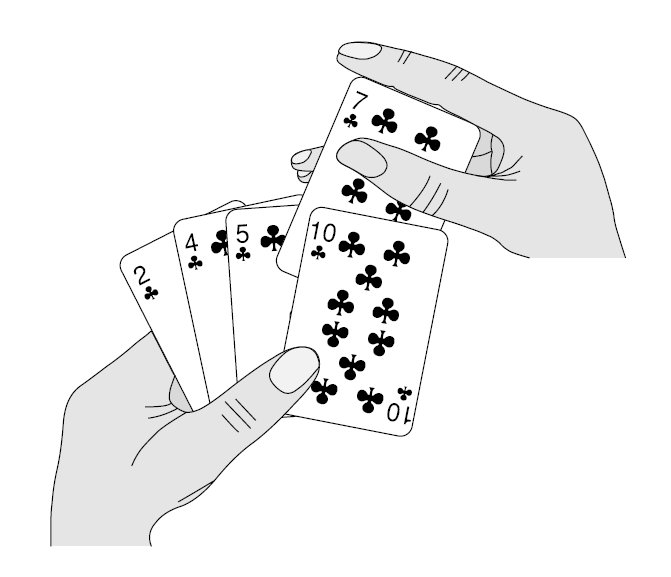
\includegraphics[scale=0.3]{insertion/cards}
    \end{figure}
    \begin{center}
        How to sort a hand of cards using insertion sort?
    \end{center}
\end{frame}
\begin{frame}
    \frametitle{Insertion Sort}
    \begin{algorithm}[H]
        \begin{algorithmic}[1]
\Statex{{\bf Algorithm} Insertion Sort($A[0..n-1]$)}
\Statex{{\bf Input:} Array $A[0..n-1]$ of orderable values}
\Statex{{\bf Output:} Array $A[0..n-1]$ in sorted in non-decreasing order}
\For{$i \gets 1$ {\bf to} $n - 1$}
    \State $key \gets A[i]$
    \State $j \gets i - 1$
    \While{$j \geq 0$ {and} $A[j] > key$}
        \State $A[j + 1] \gets A[j]$
        \State $j \gets j - 1$
    \EndWhile
    \State $A[j + 1] \gets key$
\EndFor
\end{algorithmic}

    \end{algorithm}
\end{frame}
\section{Selection Sort}
\begin{frame}
    \frametitle{Selection Sort}
    \begin{figure}[h]
        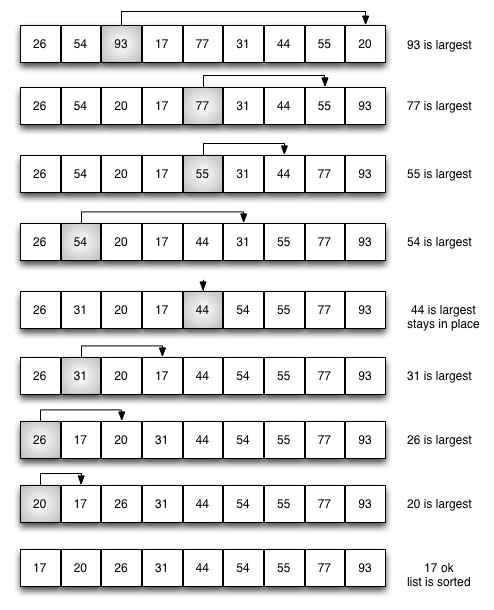
\includegraphics[scale=0.35]{selection/selection}
    \end{figure}
\end{frame}
\begin{frame}
    \frametitle{Selection Sort}
    \begin{algorithm}[H]
        \begin{algorithmic}[1]
\Statex{{\bf Algorithm} Selection Sort($A[0..n-1]$)}
\Statex{{\bf Input:} Array $A[0..n-1]$ of orderable values}
\Statex{{\bf Output:} Array $A[0..n-1]$ in sorted in non-decreasing order}
\For{$i \gets 0$ {\bf to} $n - 2$}
    \State $min \gets i$
    \For{$j \gets i + 1$ {\bf to} $n - 1$}
        \If{$A[j] < A[min]$}
            \State $min \gets j$
        \EndIf
    \EndFor
    \State $swap(A[i], A[min])$
\EndFor
\end{algorithmic}

    \end{algorithm}
\end{frame}
\section{Bubble Sort}
\begin{frame}
    \frametitle{Bubble Sort}
    \begin{figure}[h]
        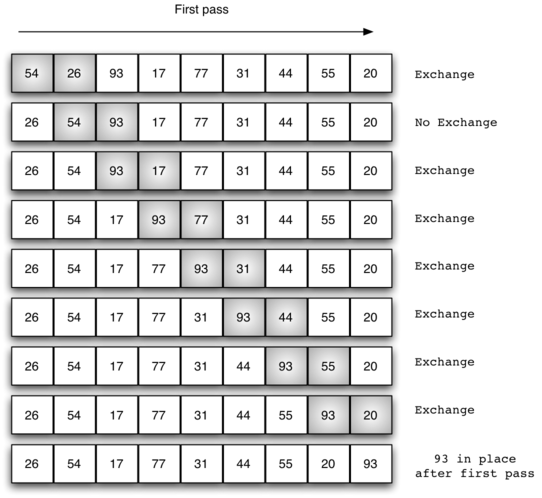
\includegraphics[scale=0.9]{bubble/bubble}
    \end{figure}
\end{frame}
\begin{frame}
    \frametitle{Bubble Sort}
    \begin{algorithm}[H]
        \begin{algorithmic}[1]
\Statex{{\bf Algorithm} Bubble Sort($A[0..n-1]$)}
\Statex{{\bf Input:} Array $A[0..n-1]$ of orderable values}
\Statex{{\bf Output:} Array $A[0..n-1]$ in sorted in non-decreasing order}
\For{$i \gets 0$ {\bf to} $n - 2$}
    \For{$j \gets 0$ {\bf to} $n - 2 - i$}
        \If{$A[j + 1] < A[j]$}
            \State $swap(A[j], A[j + 1])$
        \EndIf
    \EndFor
\EndFor
\end{algorithmic}

    \end{algorithm}
\end{frame}
\section{Merge Sort}
\begin{frame}
    \frametitle{Merge Sort}
    \begin{figure}[h]
        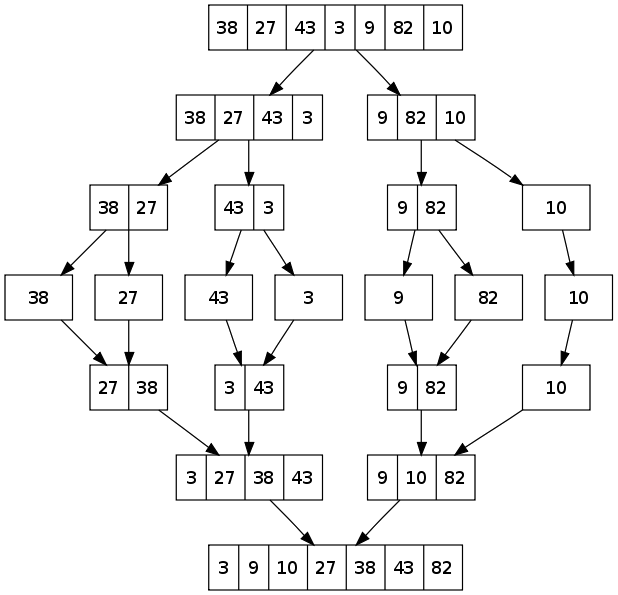
\includegraphics[scale=0.3]{merge/merge}
    \end{figure}
\end{frame}
\begin{frame}
    \frametitle{Merge Sort}
    \begin{multicols}{2}
        \begin{algorithmic}[1]
\Statex{\Call{Merge}{$A, p, q, r$}}
\State $l \gets q - p + 1$
\State $r \gets r - q$
\State Let $L[0..l]$ and $R[0..r]$ be new arrays
\For{$i \gets 0$ {\bf to} $l - 1$}
    \State $L[i] \gets A[p + i]$
\EndFor
\For{$j \gets 0$ {\bf to} $r - 1$}
    \State $R[j] \gets A[q + 1 + j]$
\EndFor
\State $L[l] \gets \infty$
\State $R[r] \gets \infty$
\State $i \gets 0$
\State $j \gets 0$
\For{$k \gets p$ {\bf to} $r$}
    \If{$L[i] \leq R[j]$}
        \State $A[k] \gets L[i]$
        \State $i \gets i + 1$
    \Else
        \State $A[k] \gets R[j]$
        \State $j \gets j + 1$
    \EndIf
\EndFor
\end{algorithmic}

        \begin{algorithmic}[1]
\Statex{\Call{Merge-Sort}{$A, p, r$}}
\If{$p < r$}
    \State $q = \floor{(p + r) / 2}$
    \State \Call{Merge-Sort}{$A, p, q$}
    \State \Call{Merge-Sort}{$A, q + 1, r$}
    \State \Call{Merge}{$A, p, q, r$}
\EndIf
\end{algorithmic}

    \end{multicols}
\end{frame}
\section{Quick Sort}
\begin{frame}{Quick Sort}
    \begin{figure}[h]
        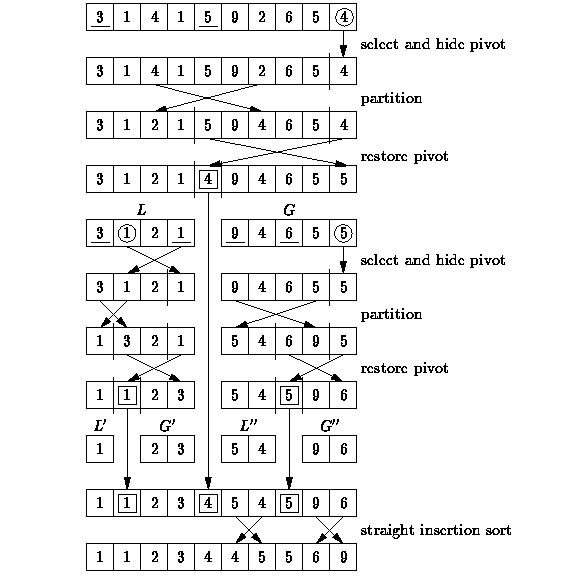
\includegraphics[scale=0.4]{quick/quick}
    \end{figure}
\end{frame}
\begin{frame}
    \frametitle{Quick Sort}
    \begin{multicols}{2}
        \begin{algorithmic}[1]
\Statex{\Call{Partition}{$A, p, r$}}
    \State $x \gets A[r]$
    \State $i \gets p - 1$
    \For{$j \gets p$ {\bf to} $r - 1$}
        \If{$A[j] < x$}
            \State $i \gets i + 1$
            \State \Call{swap}{$A[i], A[j]$}
        \EndIf
    \EndFor
    \State \Call{swap}{$A[i + 1], A[r]$}
    \State \Return $i + 1$
\end{algorithmic}

        \vfill\null
        \columnbreak
        \begin{algorithmic}[1]
\Statex{\Call{Quick-Sort}{$A, p, r$}}
\If{$p < r$}
    \State $q = $ \Call{partition}{$A, p, r$}
    \State \Call{Quick-Sort}{$A, p, q - 1$}
    \State \Call{Quick-Sort}{$A, p + 1, q$}
\EndIf
\end{algorithmic}

    \end{multicols}
\end{frame}
\section{Heap Sort}
\begin{frame}{Heap Sort}
    \begin{figure}[h]
        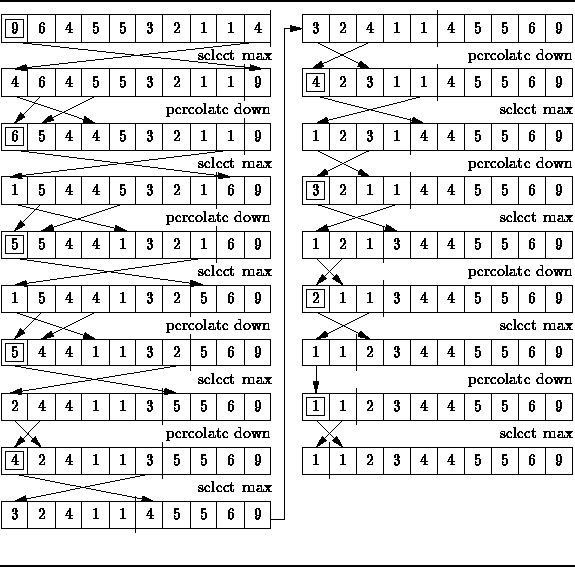
\includegraphics[scale=0.4]{heap/heap}
    \end{figure}
\end{frame}
\section{Counting Sort}
\begin{frame}{Counting Sort}
    \begin{figure}[h]
        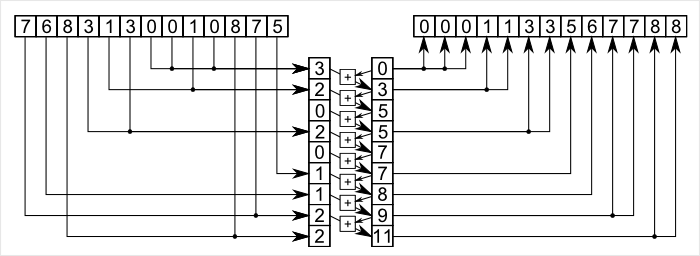
\includegraphics[width=\textwidth]{counting/counting}
    \end{figure}
\end{frame}
\section{Radix Sort}
\begin{frame}{Radix Sort}
    \begin{figure}[h]
        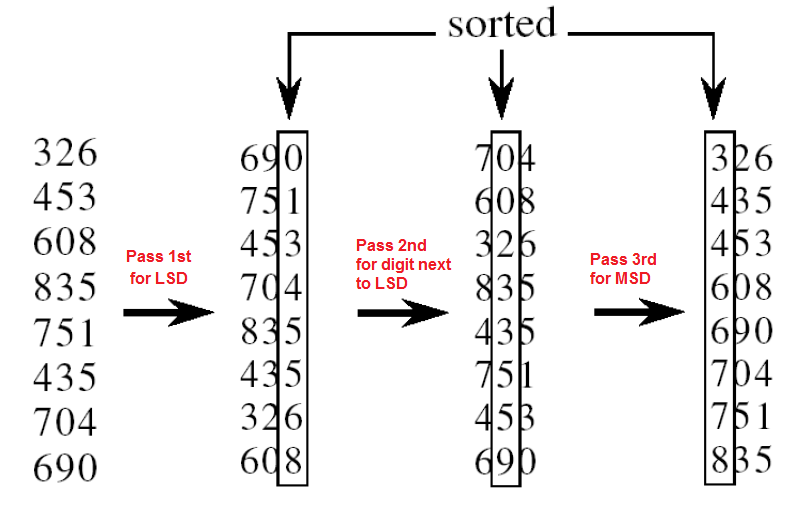
\includegraphics[width=\textwidth]{radix/radix}
    \end{figure}
\end{frame}
\section{Bucket Sort}
\begin{frame}{Bucket Sort}
    \begin{figure}[h]
        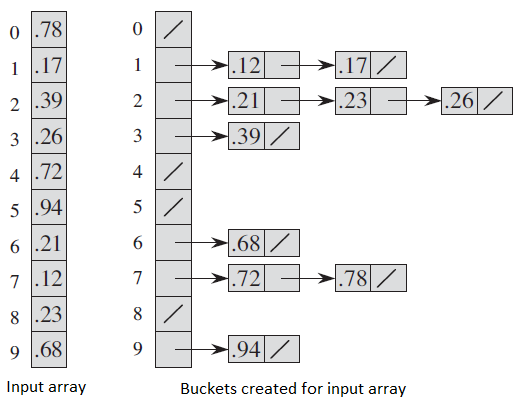
\includegraphics{bucket/bucket}
    \end{figure}
\end{frame}
\section{More Sorting Algorithms}
\begin{frame}
    \frametitle{Comparison Counting Sort}
    \begin{algorithm}[H]
        \begin{algorithmic}[1]
\Statex{{\bf Algorithm} Comparison Counting Sort($A[0..n-1]$, $S[0..n-1]$)}
\Statex{{\bf Input:} Array $A[0..n-1]$ of orderable values}
\Statex{{\bf Output:} Array $S[0..n-1]$ of $A$'s elements sorted in non-decreasing order}
\For{$i \gets 0$ {\bf to} $n - 1$}
    \State $Count[i] \gets 0$
\EndFor
\For{$i \gets 0$ {\bf to} $n - 2$}
    \For{$j \gets i + 1$ {\bf to} $n - 1$}
        \If{$A[i] < A[j]$}
            \State $Count[j] \gets Count[j] + 1$
        \Else
            \State $Count[i] \gets Count[i] + 1$
        \EndIf
    \EndFor
\EndFor
\For{$i \gets 0$ {\bf to} $n - 1$}
    \State $S[Count[i]] \gets A[i]$
\EndFor
\end{algorithmic}

    \end{algorithm}
\end{frame}
\section{Problems}
\begin{frame}{Problem A}
    Suppose that there is a restaurant and we know the arriving and leaving times of all customers on a certain day. 
    Our task is to find out the maximum number of customers who visited the restaurant at the same time.\\
    \begin{multicols}{2}
        \begin{flushleft}
            \bf{Input:}\normalfont Arriving \& Leaving\\ 
            1 6\\
            3 5\\
            2 8
        \end{flushleft}
        \vfill\null
        \columnbreak
        \begin{flushleft}
            \bf{Output:}\normalfont Number of customers\\
            3
        \end{flushleft}
    \end{multicols}
\end{frame}
\begin{frame}{Problem A - 2}
    Suppose that there is a restaurant and we know the arriving and leaving times of all customers on a certain day. 
    Our task is to find out the maximum number of customers who visited the restaurant in certain time interval.\\
    \begin{multicols}{2}
        \begin{flushleft}
            \bf{Input:}\normalfont Arriving \& Leaving\\
            3\\
            1 6\\
            3 5\\
            2 8\\
            2\\
            1 2\\
            1 8
        \end{flushleft}
        \vfill\null
        \columnbreak
        \begin{flushleft}
            \bf{Output:}\normalfont Number of customers\\
            2\\
            3
        \end{flushleft}
    \end{multicols}
\end{frame}
\begin{frame}{Problem B}
    Given $n$ events with their starting and ending times, find a schedule that includes as many events as possible.
    \begin{multicols}{2}
        \begin{flushleft}
            \bf{Input:}\normalfont Starting \& Ending\\
            7\\
            9 14\\
            23 32\\
            0 15\\
            17 29\\
            26 32\\
            13 22\\
            3 12
        \end{flushleft}
        \vfill\null
        \columnbreak
        \begin{flushleft}
            \bf{Output:}\normalfont Number of events\\
            3
        \end{flushleft}
    \end{multicols}
\end{frame}
\section{Summary}
\begin{frame}
    \frametitle{References}
    \bibliographystyle{unsrt}
    \bibliography{../ref}
\end{frame}
\end{document} 
